\section{Simplicial Abelian Groups}
\label{sec:Simplicial Abelian Groups}

There are generally two definitions of a \emph{simplicial abelian group}, an abstract one and a very explicit one. We will start with the abstract one, and immediately show in pictures what the explicit definition looks like.

\begin{definition}
	We define a category $\DELTA$, where the objects are the finite ordinals $[n] = \{0, \dots, n\}$ and maps are monotone increasing functions.
\end{definition}

There are two special kinds of maps in $\DELTA$, the so called \emph{face} and \emph{degeneracy} maps, defined as (resp.):

$$\delta_i: [n] \to [n+1], k \mapsto \begin{cases} k & \text{if } k < i;\\ k+1 & \text{if } k \geq i. \end{cases} \hspace{0.5cm} 0 \leq i \leq n+1, \text{ and}$$
$$\sigma_i: [n+1] \to [n], k \mapsto \begin{cases} k & \text{if } k \leq i;\\ k-1 & \text{if } k > i. \end{cases} \hspace{0.5cm} 0 \leq i \leq n$$

for each $n \in \N$. The nice things about these maps is that every map in $\DELTA$ can be decomposed to a composition of these maps. So in a certain sense, these are all the maps we need to consider. We can now picture the category $\DELTA$ as follows.

\begin{figure}[h!]
	\label{fig:delta_cat}
	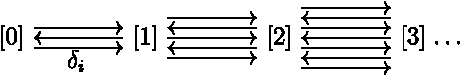
\includegraphics{delta_cat}
	\caption{The category $\DELTA$ with the face and degeneracy maps.}
\end{figure}

\todo{sAb: Epi-mono factorization of $\DELTA$}

Now the category $\sAb$ is defined as the category $\Ab^{\DELTA^{op}}$. Because the face and degeneracy maps give all the maps in $\DELTA$ it is sufficient to define images of $\delta_i$ and $\sigma_i$ in order to define a functor $F: \DELTA^{op} \to Ab$. And hence we can picture a simplicial abelian group as done in figure~\ref{fig:simplicial_abelian_group}. Comparing this to figure~\ref{fig:delta_cat} we see that the arrows are reversed, because $A$ is a contravariant functor.

\begin{figure}
	\label{fig:simplicial_abelian_group}
	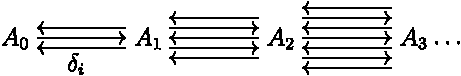
\includegraphics{simplicial_abelian_group}
	\caption{A simplicial abelian group.}
\end{figure}

Of course the maps $\delta_i$ and $\sigma_i$ in $\DELTA$ satisfy certain equations, these are the so called \emph{simplicial equations}.
\todo{sAb: Is \emph{simplicial equations} really a thing?}

\begin{lemma}
	The face and degeneracy maps in $\DELTA$ satisfy the simplicial equations, ie.:
	\begin{align}
		\delta_j\delta_i &= \delta_i\delta_{j-1}  \hspace{0.5cm} \text{ if } i < j,\\
		\sigma_j\delta_i &= \delta_i\sigma_{j-1}  \hspace{0.5cm} \text{ if } i < j,\\
		\sigma_j\delta_j &= \sigma_j\delta_{j+1} = \text{id},\\
		\sigma_j\delta_i &= \delta_{i-1}\sigma_j  \hspace{0.5cm} \text{ if } i > j+1,\\
		\sigma_j\sigma_i &= \sigma_i\sigma_{j+1}  \hspace{0.5cm} \text{ if } i \leq j.
	\end{align}
\end{lemma}
\begin{proof}
	By writing out the definitions given above.
\end{proof}

Because a simplicial abelien group $A$ is a contravariant functor, these equations (which only consist of compositions and identities) also hold in its image. For example the first equation would look like: $ A(\delta_i)A(\delta_j) = A(\delta_{j-1})A(\delta_i) $ for $ i < j$ (again note that $A$ is contravariant, and hence composition is reversed). This can be used for a explicit definition of simplicial abelien groups. In this definition a simplicial abelian group $A$ consists of a family abelian groups $(A_n)_{n}$ together with face and degeneracy maps (which are grouphomomorphisms) such that the simplicial equations hold.

\subsection{Other simplicial objects}
Of course the abstract definition of simplicial abelian group can easilty be generalized to other categories. For example $\Set^{\DELTA^{op}} = \sSet$ is the category of simplicial sets.
\todo{sAb: as example do the free abelian group pointwise}

\todo{sAb: Say a bit more (because Mueger will not like this)}